Now that we know how to plot, let's look at how to fit some curves to data and then plot the results.

\section{Mathcad: Curve Fitting}\label{sec:Mathcurvefitting}

Data sets are by definition a discrete set of points.  We can plot them, but we often want to view trends, interpolate new points and (carefully!) extrapolate for prediction purposes.  Linear regression is a powerful tool, although sometimes the data would be better fit by another curve.  Here we show how to do linear and quadratic regression.  \\

\example{ex_mathcadcurvefit1}{\po \\
\\
Consider the following data set from example \ref{ex_mathcadplot} in the previous chapter. \\

\tnr{F :=}
$\left(
\begin{array}{c}
2\\
4\\
6\\
8\\
10\\
12\\
14\\
16\\
18\\
20
\end{array}
\right) 
\cdot \tnr{kN}
\qquad 
\delta :=
\left(
\begin{array}{c}
0.82\\
1.47\\
2.05\\
3.37\\
3.75\\
4.17\\
5.25\\
5.44\\
6.62\\
7.97
\end{array}
\right) 
\cdot$ 
\tnr{mm}

A plot of the data suggests a linear relationship:

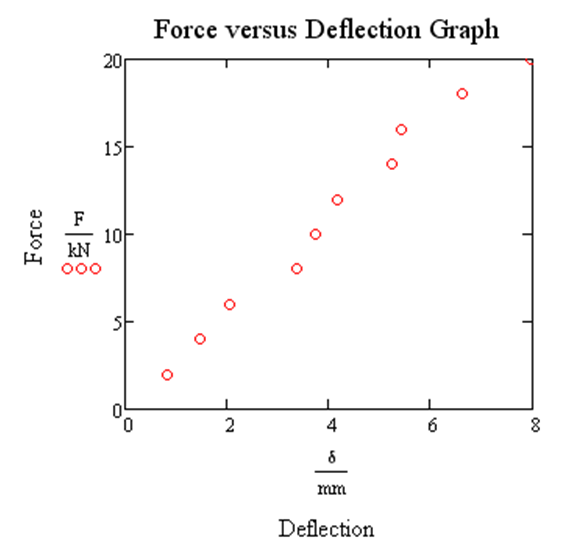
\includegraphics[scale=.8]{figures/mathcad_Fdelta_plot4.png}\\
%\drawexampleline%{ex_forceline1}

Let's find the least squares line.  We consider two methods to do this. \\

\drawexampleline%{ex_forceline2}

\underline{Method 1}\\

\index{Mathcad Functions!\tnr{slope}}
\index{Mathcad Functions!\tnr{intercept}}
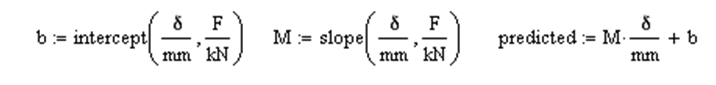
\includegraphics[scale=.9]{figures/mathcad_linear_regression.png}\\

Now put them together on the same plot:\\

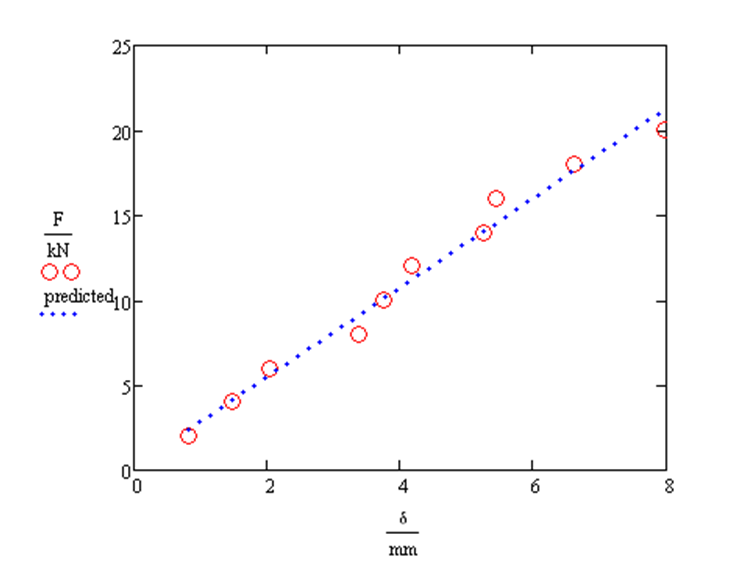
\includegraphics[scale=.6]{figures/mathcad_linear_regression_plot.png}

\drawexampleline%{ex_forceline2}

\underline{Method 2}\\
\\

\index{Mathcad Functions!\tnr{linfit}}
This method uses the command \tnr{linfit}.  It is a bit awkward here, but will be useful when we do higher order regression. 
We do have to first remove the units from our variables (a limitation of \tnr{linfit})

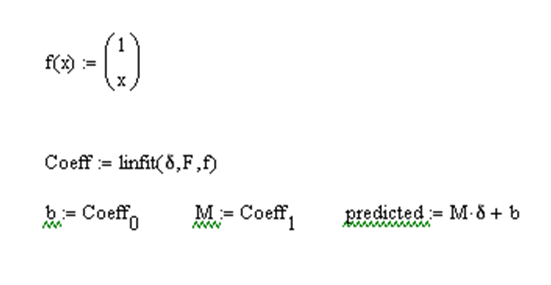
\includegraphics[scale=.9]{figures/mathcad_linfit1.png}

Now put them together on the same plot:

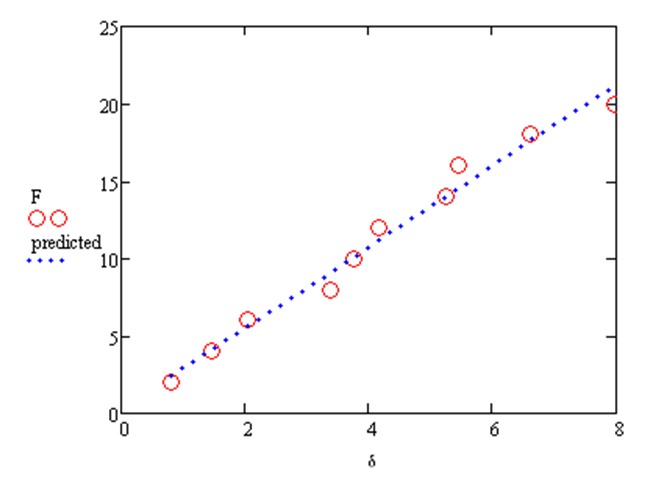
\includegraphics[scale=.6]{figures/mathcad_linfit2.png}
}\\

\example{ex_mathcadcurvefit2}{
Consider the following data set:

\tnr{Time :=}
$
\left(
\begin{array}{c}
0\\
1\\
2\\
3\\
4\\
5\\
6
\end{array}
\right) 
\quad
\tnr{Distance :=}
\left(
\begin{array}{c}
5\\
19.8\\
76.8\\
153.3\\
256.2\\
394.5\\
559.2
\end{array}
\right)
$

Plotted:

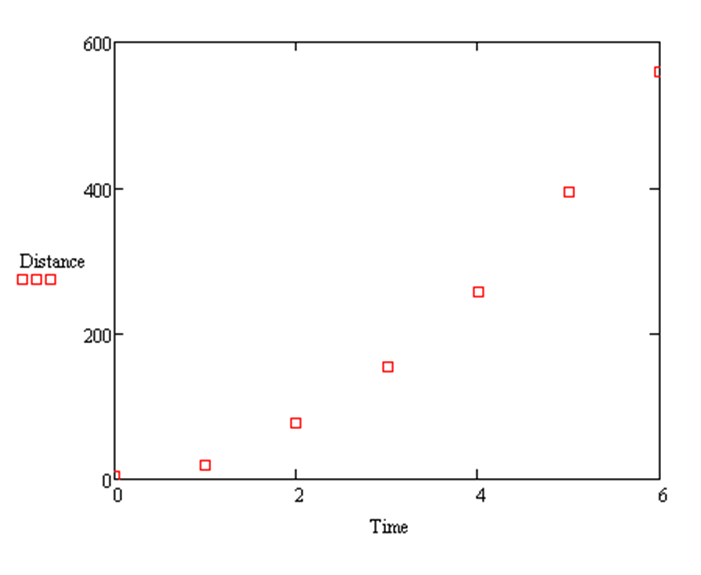
\includegraphics[scale=.6]{figures/mathcad_qfit1.png}

The plot of the data suggests a quadratic fit, i.e. a curve $y=a + bx + c x^2$.  How do we find this quadratic curve?\\

Here's how we implement this in Mathcad:

\drawexampleline
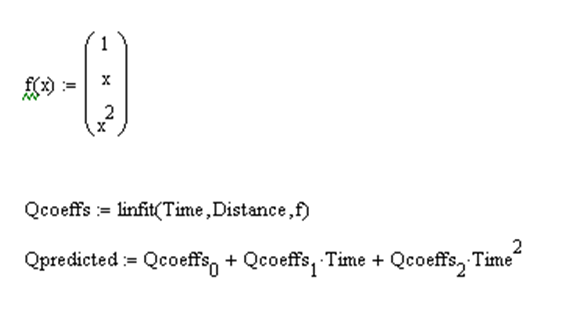
\includegraphics[scale=.9]{figures/mathcad_qfit2.png}

Now plot them together:

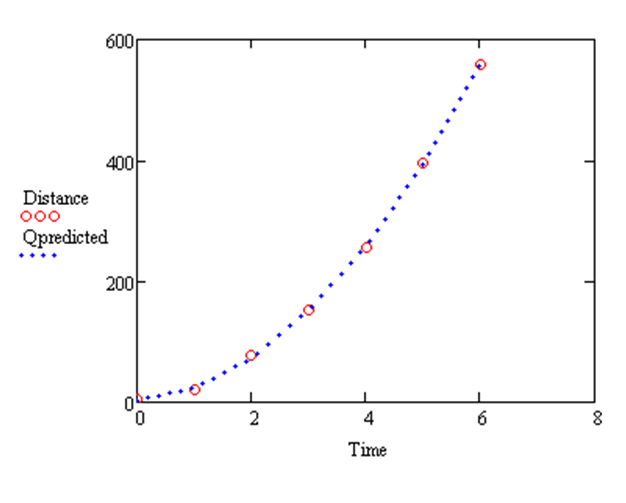
\includegraphics[scale=.6]{figures/mathcad_qfit3.png}

We can compute the R-squared value to see the correlation between \tnr{Distance} and \tnr{Qpredicted}.

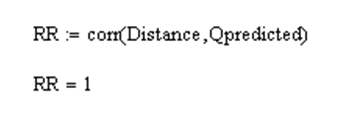
\includegraphics[scale=.6]{figures/mathcad_qfit4.png}

\index{Mathcad Functions!\tnr{corr}}
\tnr{RR=1} means a great fit.}

\newpage
\printexercises{exercises/16_exercises}